\documentclass[leqno]{article}
\usepackage{verbatim}
\usepackage{array}
\usepackage{listings}
\usepackage{fancyvrb}
\usepackage{enumitem}

\usepackage[utf8]{inputenc}
\usepackage[T1]{fontenc}
\usepackage{textcomp}
\usepackage{multicol} \usepackage{mathtools}
\usepackage{amsmath}
\usepackage{wrapfig}
\usepackage{amssymb}
\usepackage{amsmath,amsfonts,amssymb,amsthm,epsfig,epstopdf,titling,url,array}
\usepackage{hyperref}
\usepackage{eso-pic}
\usepackage{pgf}
\usepackage{tikz}
\usepackage{tikz-cd}
\usepackage{graphicx}

% figure support
\usepackage{import}
\usepackage{xifthen}
\pdfminorversion=7
\usepackage{pdfpages}
\usepackage{transparent}
\usepackage{xcolor}

% geometry
\usepackage{geometry}
\geometry{a4paper, margin=1in}

% paragraph length
\setlength{\parindent}{0em}
\setlength{\parskip}{1em}

\newtheorem*{theorem}{Theorem}
\newtheorem*{lemma}{Lemma}
\newtheorem*{proposition}{Proposition}
\newtheorem*{definition}{Definition}
\newtheorem*{observation}{Observation}

\newcommand{\incfig}[1]{%
\center
\def\svgwidth{0.9\columnwidth}
\import{./figures/}{#1.pdf_tex}
}
\newcommand{\incimg}[1]{%
\center
\includegraphics[width=0.9\columnwidth]{images/#1}
}
\pdfsuppresswarningpagegroup=1

\title{Estado Sólido}
\author{Abel Doñate Muñoz}
\date{}

\begin{document}
\maketitle
\tableofcontents
\newpage

\section{Estructura cristalina}

\subsection{Redes cristalinas, base primal y dual}
\begin{definition}[Red] Una red es un conjunto infinito de puntos generado por el set de vectores
   \[
  R = n_1 \overline{a} + n_2 \overline{b} + n_3 \overline{c} \qquad n_i \in \mathbb{Z}
  \] 
\end{definition}

\begin{definition}[Celda unidad] Una celda unidad es una region de el espacio que puede teselar el espacio. Si sólo contiene un punto de la red, se dice que es primitiva.
\end{definition}

\begin{definition}[Célula de Wigner-Seitz] Dado un punto de la red, la celda de Wigner-Seitz es el espacio de los puntos más cercanos a el punto que a cualquier otro punto.
\end{definition}

\begin{definition}[Base] Una base de un sistema cristalino es un conjunto de tres vectores linealmente independientes $\{\overline{a}, \overline{b}, \overline{c}\}$. Su base dual $ \{\overline{a}^*, \overline{b}^*, \overline{c}^*\}$ se puede calcular de las siguientes maneras:
\[
  a^* = \frac{b\times c}{V}, \quad b^* = \frac{c\times a}{V}  , \quad c^* = \frac{a\times b}{V} \qquad \text{ó}  \qquad (\overline{a}^*, \overline{b}^*, \overline{c}^*)=\begin{pmatrix} \overline{a}^T\\\overline{b}^T\\\overline{c}^T \end{pmatrix} ^{-1}
\] 
\end{definition}
Formalmente la base dual debería ir multiplicada por $2\pi$ por estar en el espacio de las $k$, pero en estos apuntes multiplicaremos por  $2\pi$ cuando haga falta.

Cada red primal tiene su red dual definida de la misma forma que definimos red, pero con combinaciones enteras de los vectores duales (multiplicados por $2\pi$). Cada red de Bravais transforma en una red de Bravais.

\subsection{Clasificación de redes cristalinas}
\subsubsection{Símbolo de Pearson}
El símbolo de Pearson consiste en dos letras y un número con el formato $aA0$.
La primera letra especifica la familia del cristal. La segunda el tipo de centro. El número final indica la cantidad de átomos en la célula unidad.

\begin{minipage}{0.45\textwidth}
\begin{center}
\begin{tabular}{|l|l|}
\hline
$a$ & triclínica  \\ \hline
$m$ & monoclínica\\ \hline
$o$ & ortorómbica\\ \hline
$t$ & tetragonal \\ \hline
$h$ & hexagonal\\ \hline
$c$ & cúbica \\ \hline
\end{tabular}
\end{center}
\end{minipage}
\begin{minipage}{0.45\textwidth}
\begin{center}
\begin{tabular}{|l|l|}
\hline
$P$ & Primitiva \\\hline
$S$ & Centrada en una cara\\\hline
$I$ & Centrada en el cuerpo\\\hline
$R$ & Centrada romboidal\\\hline
$F$ & Centrada en las caras \\\hline
\end{tabular}
\end{center}
\end{minipage}

Esto nos proporciona las 14 posibles redes de Bravais
\begin{center}
\begin{tabular}{|c|c|c|c|c|c|}
\hline
Triclínico & Monoclínico & Ortorómbico & Tetragonal & Hexagonal & Cúbico \\\hline
$aP$ &  $mP, mS$ &  $oP, oS, oF, oI$ &  $tP, tI$ &  $hP, hR$ &  $cP, cF, cI$ \\\hline
\end{tabular}
\end{center}

\subsubsection{Grupos de simetría}
Pa otro dia jeje

\subsection{Descripción de las redes cristalinas más comunes}
\subsubsection{FCC}


\section{Tema 2 supongo}
En esta sección veremos tres modelos diferentes de propagación de ondas por la red cristalina.
\begin{enumerate}[topsep=-6pt, itemsep=0pt]
  \item \textbf{Dulong-Petit} Los átomos vibran independientemente. Clásico. $C_v$ independiente de la temperatura.
  \item \textbf{Einstein} Los átomos vibran independientemente. Cuántico. $C_v$ coincide para temperaturas altas pero falla para bajas.
  \item \textbf{Debye} Los átomos vibran dependiendo del vecino próximo. Cuántico. Aproximación dispersión lineal. $C_v$ refleja la dependencia cúbica experimental para temperaturas bajas.
\end{enumerate}

La gráfica de los modelos teóricos es

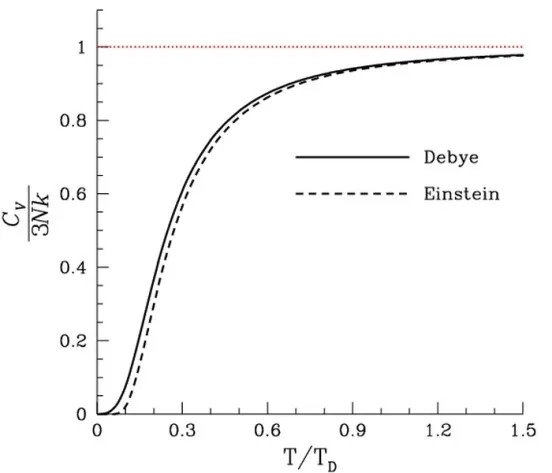
\includegraphics[width=\textwidth]{figures/comparisoncv.jpg}

\subsection{Dulong-Petit model}
\subsection{Modelo de Einstein}
Este modelo está basado en el oscilador harmónico cuántico. Si suponemos que en la red cristalina se comportan todos los átomos como osciladores harmónicos cuánticos, entonces podemos calcular su función grancanónica
\[
  E_n = \hbar \omega (n+\frac{1}{2}) \quad \Rightarrow \quad Z_1 = \frac{1}{2 \sinh(\frac{\beta \hbar \omega }{2})}, \quad \langle E_1 \rangle = - \frac{\partial }{\partial \beta } \ln Z_1 = \frac{\hbar\omega }{2} \coth \left( \frac{\beta \hbar \omega }{2} \right) 
\] 
Pero debemos tener en cuanta que hay 3 dimensiones y $N$ partículas, por lo que debemos multiplicar por 3 en la energía media. Ahora podemos calcular también la capacidad calorífica $C_v$.
 \[
\langle E\rangle = \frac{3}{2} N \hbar \omega \coth \left( \frac{\beta \hbar \omega  }{2} \right) \quad \Rightarrow \quad
C_v = \frac{\partial \langle E\rangle}{\partial T}  = 3Nk_B (\beta \hbar \omega )^2 \frac{e^{\beta \hbar \omega }}{(e^{\beta \hbar \omega }-1)^2}
\] 
Definimos ahora $T_E = \frac{\hbar \omega_E}{k_B}$. Vamos a ver que pasa en los limites de temperatura.

\begin{itemize}[topsep=-6pt, itemsep=0pt]
  \item Si  $T\gg T_E \quad \Rightarrow \quad C_v = 3Nk_b$
  \item Si  $T\ll T_E \quad \Rightarrow \quad C_v = 3Nk_b (\frac{T_E}{T})^2 \frac{1}{\sinh ^2(\frac{T_E}{2T})}$
\end{itemize}

Observamos que, como es de esperar, para temperaturas altas el modelo cumple la ley de Dulong-Petit, pero para bajas no cumple la expectativa experimental de $C_v \sim  T^3$.


\subsection{Modelo de Debye}
Comenzamos analizando una cadena de átomos cuya única fuerza entre ellos es modelizable mediante la ley de Hook con una constante de muelle $k_s$. Si  $r_n$ es la posición de cada átomo y $x_n = r_n-na$ el desplazamiento con respecto al punto de equilibrio tenemos:
 \[
F_n =m\ddot{x}_n = k_s(x_{n+1}+x_{n-1}-2x_n)
\] 
Suponemos (oh, sorpresa) que la solución es una oscilación armónica de la forma $x_n = A e^{i(kna-\omega t)}$. Calculamos ahora como debe se la $\omega $ en función de la $k$.
 \[
   -m\omega ^2 Ae^{i(kna-\omega t)} = k_sAe^{i(kna-\omega t)}(e^{ika}+e^{-ika}-2) = -4k_s \sin^2\left( \frac{ka}{2} \right)  \Rightarrow \boxed{\omega = 2 \sqrt{\frac{k_s}{m}}\left|\sin \left( \frac{ka}{2} \right) \right| }
\] 
Lo que se conoce como ecuación de dispersión. Observamos que en la zona cercana a $k=0$ podemos aproximar a una dispersión casi lineal  $\omega =\nu k$. Si tomamos esta aproximación hasta una frecuencia de corte dada $\omega _D$, podemos calcular esta frecuencia de corte como
\[
  3N = \int_0^{\omega _D} 3g(\omega )d\omega =\int_0^{\omega _D}3 \frac{V}{2\pi^2\nu^3}\omega ^2 d\omega = \frac{V}{2\pi^2 \nu^3}\omega _D^3 \Rightarrow \boxed{\omega _D = \sqrt[3]{\frac{6\pi^2\nu^3N}{V}} }
\] 
donde hemos contado cada partícula y cada estado 3 veces y hemos usado
\[
\omega = \nu k, \qquad g(k)=\frac{V}{2\pi^2}k^2, \qquad g(\omega )= \frac{V}{2\pi^2 \nu^3}\omega ^2
\]
Calculamos ahora la energía media para calcular la capacidad calorífica
\begin{align*}
  \langle E \rangle &= \int_0^{\omega _D}\hbar \omega 3g(\omega )\left( \frac{1}{e^{\beta \hbar \omega }-1} +\frac{1}{2} \right) d\omega  = E_0 + \frac{3V\hbar }{2\pi^2\nu^3} \int_0^{\omega _D}\frac{\hbar \omega ^3}{e^{\beta \hbar \omega }-1} d\omega \\
	   & (x=\frac{\hbar \omega }{k_B T}), \quad T_D := \frac{\hbar \omega }{k_B} \quad   \Rightarrow  \boxed{\langle E \rangle = \frac{3Vk_B^4T^4}{2\pi^2\nu^3\hbar ^3}\int_0^{\frac{T_D}{T}}\frac{x^3}{e^x-1}dx }
\end{align*}
Estudiamos ahora que pasa con capacidad calorífica $C_v = \frac{\partial \langle E \rangle }{\partial T}$ en los extremos:
\begin{itemize}[topsep=-6pt, itemsep=0pt]
  \item Si $T\gg T_D \quad \Rightarrow \quad \langle E \rangle \sim 3Nk_BT \quad \Rightarrow \quad C_v \sim  3Nk_B $
  \item Si $T\ll T_D \quad \Rightarrow \quad \langle E \rangle \sim  \frac{3\pi^4Nk_BT^4}{5T_D^3}\quad\Rightarrow \quad C_v \sim  \frac{12\pi^4}{5}Nk_B \left( \frac{T}{T_D} \right)^3 $
\end{itemize}
donde hemos usado $\int_0^\infty \frac{x^3}{e^x-1}dx=\frac{\pi^4}{15}$.

Observamos como este modelo si que refleja la dependencia cúbica observada experimentalmente.







\end{document}
